\documentclass[a4paper]{article}

\usepackage[swedish]{babel}
\usepackage[T1]{fontenc}
\usepackage[utf8]{inputenc}
\usepackage{graphicx}
\usepackage{array}
\usepackage[nottoc,notlot,notlof]{tocbibind}

\begin{document}

\pagenumbering{gobble}
\title{ \textbf{Projektplan DAT290} \\ Datatekniskt projekt \\ Grupp 12}
\author{Daniel Ferreira, Jakob Wik, Erik Söderpalm,\\Christoffer Kaltenbrunner, Lam Nguyen}
\date{2019-09-12}
\maketitle

\newpage
\tableofcontents

\newpage
\pagenumbering{arabic}

\section{Syfte}
\label{sec:syfte}

Projektet syftar främst till att göra vår kund nöjd, vilket innebär att en produkt ska utvecklas och denna också uppnå de produktkrav som ställts av kunden.\footnote{Se tabell \ref{tabell:krav} för en detaljerad lista över dessa krav.}

Det syftar även till att firman ska etablera sig på marknaden för larm- och låssystem. Detta är av intresse då säkerhetsbranschen växer till följd av att allt fler svenskar upplever att brottsligheten ökar. Branschen ökade med cirka 8 procent från 2017 till förra året, då den omsatte 39 miljarder kronor\cite{sverigesRadio}.

För att uppnå våra syften har projektgruppen satt upp ett antal mål som ska nås. Som resultat av att ha uppfyllt målen kommer firman att ha en högkvalitativ produkt på marknaden för larm- och låssystem.

\section{Mål}
\label{sec:mål}

Målet med projektet är att utveckla ett larm- och låssystem med hjälp av en mikrokontroller och ett antal periferienheter.
Larm- och låssystemet består av ett grundsystem med ett antal tilläggsfunktioner.

Grundsystemet utgörs av ett dörrlarm och ett rörelselarm. Dessutom ska en störenhet för teständamål konstrueras. Inställningarna för enheterna kan konfigureras via en centralenhet.

Tilläggsfunktionerna delas in i två delar: (1) viktiga funktioner och (2) mindre viktiga funktioner. De viktiga funktionerna omfattar en funktion att slå om från produktionsläge till testläge för enklare test av periferienheterna samt en funktion som gör systemet självlärande.  De mindre viktiga funktionerna omfattar RSA-kryptering av meddelanden som skickas i systemet samt en upp-seendeväckande larmsignal.
I första hand ska de viktiga funktionerna utvecklas.

\section{Bakgrund}
\label{sec:bakgrund}

Som tidigare nämnt ökade efterfrågan för inbrottslarm i Sverige mellan 2016 och 2017 med 8 procent. Detta tyder på att det finns ett växande behov av produkter inom larm- och säkerhetsbranschen.

Ett vanligt larmsystem består av en centralstation där inställningar, larm-status och återställning av larmet hanteras, samt ett antal periferienheter som dörrlarm, fönsterlarm och rörelsedetektorer. Periferienheterna skickar kontinuer-ligt information till centralstationen som i sin tur tolkar informationen och uppdaterar larmstatusen.

\begin{description}
\item [Dörrlarm] Dörrlarm består vanligtvis av en sensor och en magnet som håller kontakten för att larmet inte ska aktiveras. Dessa har kontakt hela tiden när dörren är stängd, men så fort sensorn tappar kontakt med magneten, till exempel om dörren öppnas, skickas en signal till centralstationen och larmet aktiveras.
\item [Fönsterlarm] Fönsterlarm består av vibrationssensorer som är fastsatta på fönstret. Om vibrationerna för sensorn når över en bestämd tröskel, till exempel om fönstret krossas, skickar vibrationssensorn signaler till central-enheten som aktiverar ett larm.
\item [Rörelsedetektor] Rörelsedetektorer använder sig av ultraljud. Tiden det vid en viss tidpunkt tar för ljudvågorna att studsa tillbaka till sensorn beräknas. Denna jämförs med tiden det tagit för ljudvågorna att vid en tidigare tidpunkt studsa tillbaka till sensorn. Rörelsedetektorn kan då bedömma om något har rört sig inom dess övervakningsområde.
\end{description}

\section{Systemöversikt}
\label{sec:systemöversikt}

Larmsystemet är autonomt och består av en uppsättning datoriserade enheter. En persondator ansluts till systemet för att ta emot larmsignaler.

Systemet består av en centralenhet och ett valbart antal anslutna periferi-enheter med sensorer av olika typer. Periferienheterna sköter övervakandet av intressanta lägen, så som fönster och dörrar, och skickar en larmsignal till centralenheten då de indikerar misstänksam aktivitet. Centralenheten övervakar i sin tur periferienheterna och skickar en larmsignal till den anslutna datorn då larm har lösts ut, eller om någon av periferienheterna oväntat kopplats ur. Konfiguration och kalibrering av systemet kan utföras på centralenheten eller genom ansluten dator.

\begin{figure}
\centering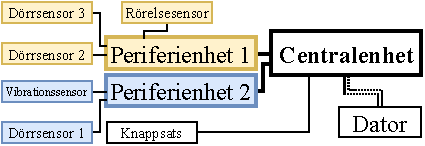
\includegraphics[width=0.8\textwidth]{figurer/systemoversiktfigur1.pdf}
\caption{Översikt av larmsystemet.}
\label{figur:översikt}
\end{figure}

I figur \ref{figur:översikt} illustreras ett exempel på en installation av larmsystemet. Det har här installerats i ett hus där periferienhet 2 övervakar huvudingången och hallfönstret, och periferienhet 1 övervakar bakingången, garagedörren och veran-dan. Centralenhetens knappsats är placerad i anslutning till huvudingången för snabb tillgång till på- och avlarmning.

Systemet har inbyggda säkerhetsmekanismer för att hantera avvikelser. Skul-le någon periferienhet eller sensor gå sönder eller oväntat kopplas ifrån så känner centralenheten av detta och skickar larmsignal.

I tabell \ref{tabell:krav} visas en sammanställning av de krav kunden ställt på produkten.

\subsection*{Sensorer}
\begin{description}
\item[Dörrsensorn] är av magnetisk typ och består av två delar, en fästs på dörren och den andra på dörrkarmen. De indikerar när dörren öppnas och mag-neterna inte längre känner av varandra.
\item[Rörelsesensorn] använder sig av ultraljud för att övervaka ett område, och indikerar när rörelsen i området överstiger ett visst gränsvärde. Gränsvär-det går att ställa in och kalibrera genom centralenheten för att få en lämplig nivå av känslighet.
\item[Vibrationssensorn] är mekanisk och känner av vibration och rörelse\cite{vibrationsSensor}. Den placeras på objektet eller på ett objekt som har direkt fysisk kontakt med objektet. Sensorn indikerar rörelse då den känner av ett värde som överstiger ett gränsvärde. Gränsvärdet ställs in direkt på sensormodulen.
\end{description}


\begin{table}[h]
\centering
\begin{tabular}{| l | l | p{0.8\linewidth}|}
\hline
\textbf{ID} & \textbf{Komponent} & \textbf{Beskrivning} \\ \hline
K01 & P1 & Om en dörr stått öppen en viss tid ska enheten larma lokalt. Efter ytterligare en tid ska enheten larma centralenheten. \\ \hline
K02 & C & När larmet gått ska det fortsätta tills en fyrsiffrig kod matas in på knappsatsen vid centralenheten. \\ \hline
K03 & P1 & Flera dörrar ska kunna larmas med samma enhet. \\ \hline
K04 & N & Nätverket ska ha stöd för flera dörrlarmsenheter samtidigt. \\ \hline
K05 & P1 & Antalet dörrar för en dörrenhet ska kunna konfigureras när enheten startas genom  USART,  via  CAN  från  centralenheten  eller genom strömbrytare. \\ \hline
K06 & P1 & Larmet för enskilda dörrar ska kunna inaktiveras och aktiveras genom att på centralenheten ange en fyrsiffrig kod och ett ID för dörren. Om en dörr är olarmad ska en grön lysdiod lysa. Via centralenheten ska man kunna konfigurera hur länge varje dörr tillåts vara öppen innan larmet går. \\ \hline
K07 & P2 & Enheten ska använda en ultraljudsbaserad avståndsmätare som rörelselarm. Enheten ska larma centralenheten om någon eller något rör sig inom dess räckvidd. \\ \hline
K08 & P2 och C & Från  centralenheten  ska  man  kunna  justera  känsligheten  för avståndsmätaren på periferienhet 2, samt kalibrera den. \\ \hline
K09 & P2 & Enheten ska använda en vibrationssensor, som kan monteras på en fönsterruta, som rörelselarm. Enheten ska larma centralenheten om fönsterrutan krossas. \\ \hline
K10 & S & Störenheten ska skicka stora volymer data på CAN-bussen. Volymen data som skickas ska kunna justeras. \\ \hline
K11 & C & När ett larm uppstår ska centralenheten kommunicera det till en ansluten PC via  USART. \\ \hline
K12 & C & När  systemet  startas  ska  centralenheten  kunna  konfigureras  via  USART  så  att  den känner till vilka enheter som finns anslutna och hur de är konfigurerade. \\ \hline
K13 & C & Centralenheten ska larma ifall någon periferienhet går sönder eller kopplas från nätverket. \\ \hline
\end{tabular}
\caption{Krav på grundsystemet utifrån kundens beskrivning. P1 står för periferienhet 1 (dörrlarm), P2 för periferienhet 2 (rörelselarm), S för störenhet, C för centralenhet och N för nätverk.}
\label{tabell:krav}
\end{table}

\section{Resursplan}
\label{sec:resursplan}
Projektets ansvarområden är uppdelat till medlemmarna enligt lista nedan: 
\begin{itemize}
\item Christoffer Kaltenbrunner \texttt{[chrkalt@student.chalmers.se]} 
	\begin{itemize}
	\item Gruppledare: Ansvarar för kommunikationen inom gruppen och mel-lan gruppen och externa kontakter. Kallar till och leder gruppmöten.
	\item Testansvarig: Ansvarar för olika tester som behöver genomföras på mjuk- och hårdvara, ser till att tillräckligt med tid ägnas åt test och att testerna är väldokumenterade. 
	\end{itemize}
\item Daniel Ferreira \texttt{[danfer@student.chalmers.se]}
	\begin{itemize}
	\item Tekniskt dokumentationsansvarig: Ser till att kod är väl kommen-terad och uppmärksammar gruppen ifall det uppstår problem.
	\item Kodstandardansvarig: Ansvarar för kodutveckling, ser till att koden förljer standarder för struktur, namn och så vidare för att uppnå kodkvalitet.
	\end{itemize}
\item Thanh Lam Nguyen \texttt{[thanhl@student.chalmers.se]}
	\begin{itemize}
	\item Resursansvarig: Ser till att hårdvara och olika verktyg som används för kommunikation, versionshantering och så vidare finns tillgängliga och fungerar väl.
	\end{itemize}
\item Erik Söderpalm \texttt{[eriks@student.chalmers.se]}
	\begin{itemize}
	\item Administrativt dokumentationsansvarig: Ansvarar för att mötesproto-koll, oppositionsrapport, planeringsrapport och så vidare förs och skickas in i tid. 
	\end{itemize}
\item Jakob Wik \texttt{[wikj@student.chalmers.se]}
	\begin{itemize}
	\item Planeringsansvarig: Håller reda på de olika delmål gruppen arbetar mot, kommunicerar med de andra medlemmarna om hur arbetet går och uppmärksammar vid behov gruppen ifall det inte görs framsteg mot något mål, så att gruppen kan omfördela arbetsinsatser.
	\end{itemize}
\end{itemize}

Alla veckomöten och testtillfällen kommer att hållas i rum EG-4213 i EDIT-huset i mån av lokaltillgänglighet, med reservation för ändring. Grupprum som kan användas vid exempelvis gruppkodning, småmöten och liknande, finns till-gängliga för bokning i EDIT-huset vid behov.

Hårdvara för projektet:
\begin{itemize}
	\item 3x MD-407-kort
	\item 1x Ultraljud avståndsmätare, HC-SR04
	\item 1x Vibrationssensor, "Flying Fish" SW-18010P
	\item 1x Keypad
	\item 1x 7-segmentsdisplay
	\item 2x 4-polig RJ-11 kabel (används för CAN-bussen)
	\item 1x RJ-11 förgrening
	\item 2x Tiopolig flatkabel
	\item 3x USB-kabel
	\item 1x Kopplingsplatta
	\item Kopplingskablar
\end{itemize}

Hårdvaran är inlåst i ett säkerhetsskåp i rum EG-4213. Skåpet låses upp med PIN-kod som alla gruppmedlemmar har tillgång till. Utöver ovan nämnd hårdvara finns det möjlighet att använda annan utrustning, till exempel dörrsen-sor.
Git används som versionshanteringssystem för projektet. Ett privat fjärrepo på GitHub har skapats och delats med hela gruppen. All projektrelaterad kod och dokumentation kommer att finnas där.

\section{Milstolpar}
\label{sec:milstolpar}

\begin{table}[h]
\centering
\begin{tabular}{| l | l | l |}
\hline
\textbf{ID} & \textbf{Beskrivning}         & \textbf{Datum} \\ \hline
M01         & Skapa GitHub-repo            & 2019-09-05     \\ \hline
M02         & Projektplan lämnad till kund & 2019-09-13     \\ \hline
M03         & Prototyp av grundsystem klar & 2019-09-27     \\ \hline
M04         & Rapportutkast 1 klart        & 2019-10-04     \\ \hline
M05         & Tilläggsfunktioner klara     & 2019-10-04     \\ \hline
M06         & Rapportutkast 2 klart        & 2019-10-18     \\ \hline
M07         & Dokumentation och förbättring
              av koden                     & 2019-10-18     \\ \hline
M08         & Demonstrationsförberedelser  & 2019-10-25     \\ \hline
M09         & Projektrapport lämnad till
              kund                         & 2019-10-31     \\ \hline
M10         & Demo                         & 2019-10-31     \\ \hline
\end{tabular}
\caption{Milstolpar för projektet och tillhörande datum då de senast ska vara klara.}
\end{table}

\section{Aktiviteter}
\label{sec:aktiviteter}

I tabell \ref{tabell:aktiviteter} ges en aktivitetslista med ungefärlig tidsåtgång som varje aktivitet kräver.

Läsa igenom dokumentation för MD-407 och resterande hårdvara uppskattas till att inte ta mer än en halv arbetsdag.

Gruppen har för avsikt att träffas över ett projektmöte i veckan. På dessa möten ska projektet ses över och vad alla gruppmedlemmar har producerat eller ändrat senaste veckan.

De första två veckorna förmodas nästan all tid gå åt att skriva projektplanen, detta innebär att alla lägger cirka 20 timmar var.

Planen är att vara klara med grundsystemet inom två veckor från den första utvecklingsdagen\footnote{Med \textit{utveckling} menas hela processen från design till kodning.}. Under dessa två veckor ska systemet även testas och tillhörande testfall skrivas. Övrig tid under dessa veckor ägnas åt rapport-skrivningen.

När grundsystemet är färdigutvecklat har gruppen för avsikt att utveckla tilläggsfunktioner över den nästföljande veckan samt utföra tester på dessa.

Dokumentation och kodförbättring förmodas ta cirka en arbetsvecka.

Andra utkastet av rapporten uppskattas till att ta cirka halva tiden som gick åt att skriva det första, då det endast är några få korrigeringar som behöver göras.

Demoförberedelserna estimeras till att ta cirka två dagars arbetstid att genomföra. Demonstrationen kommer i sig ta cirka två timmar och alla i projekt-gruppen är närvarande.

Slutligen uppskattar gruppen att slutrapporten endast kräver några enkla korrigeringar, som beräknas ta cirka två dagars arbetstid.

Gruppen har för avsikt att på de veckoliga mötena dela ut arbetsuppgifter utifrån den rådande situationen. Alla medlemmar är eniga om att detta system är fördelaktigt, eftersom det är svårt att bestämma vilka aktiviteter som ska utföras av vem redan nu. Aktivitetslistan är därmed översiktlig. Dessutom finns en buffert på 110 timmar som kan fördelas utifrån behov.

\begin{table}[t]
\centering
\begin{tabular}{| l | l | l |}
\hline
\textbf{ID} & \textbf{Beskrivning} & \textbf{Tidsåtgång} \\ \hline
A01 & Läsa dokumentation & 20 h \\ \hline
A02 & Projektmöten (1-1.5 h/vecka, 8 veckor, 5 personer) & 50 h \\ \hline
A03 & Skapa GitHub-repo & 1 h \\ \hline
A04 & Skriva projektplan & 100 h \\ \hline
A05 & Utveckling av grundsystemet & 150 h \\ \hline
A06 & Rapportutkast 1 & 100 h \\ \hline
A07 & Skriva testfall & 10 h \\ \hline
A08 & Tester av grundsystemet & 50 h \\ \hline
A09 & Utveckling av tilläggsfunktioner & 100 h \\ \hline
A10 & Tester av tilläggsfunktioner & 50 h \\ \hline
A12 & Dokumentation och kodförbättring & 100 h \\ \hline
A13 & Rapportutkast 2 & 50 h \\ \hline
A14 & Demoförberedelser & 50 h \\ \hline
A15 & Demo (2 h/person, 5 personer) & 10 h \\ \hline
A16 & Slutrapport & 50 h \\ \hline
A17 & Övrigt & 110 h \\ \hline
\end{tabular}
\caption{Aktivitetslista och den uppskattade tidsåtgången för varje aktivitet i totala mantimmar}
\label{tabell:aktiviteter}
\end{table}

\section{Tidsplan}
\label{sec:tidsplan}

En skiss på en Ganttbaserad tidsplan för projektet presenteras i figur \ref{figur:tidsplan}. Tids-planen bygger på aktiviterna i tabell \ref{tabell:aktiviteter}.

\begin{figure}[h]
\centering
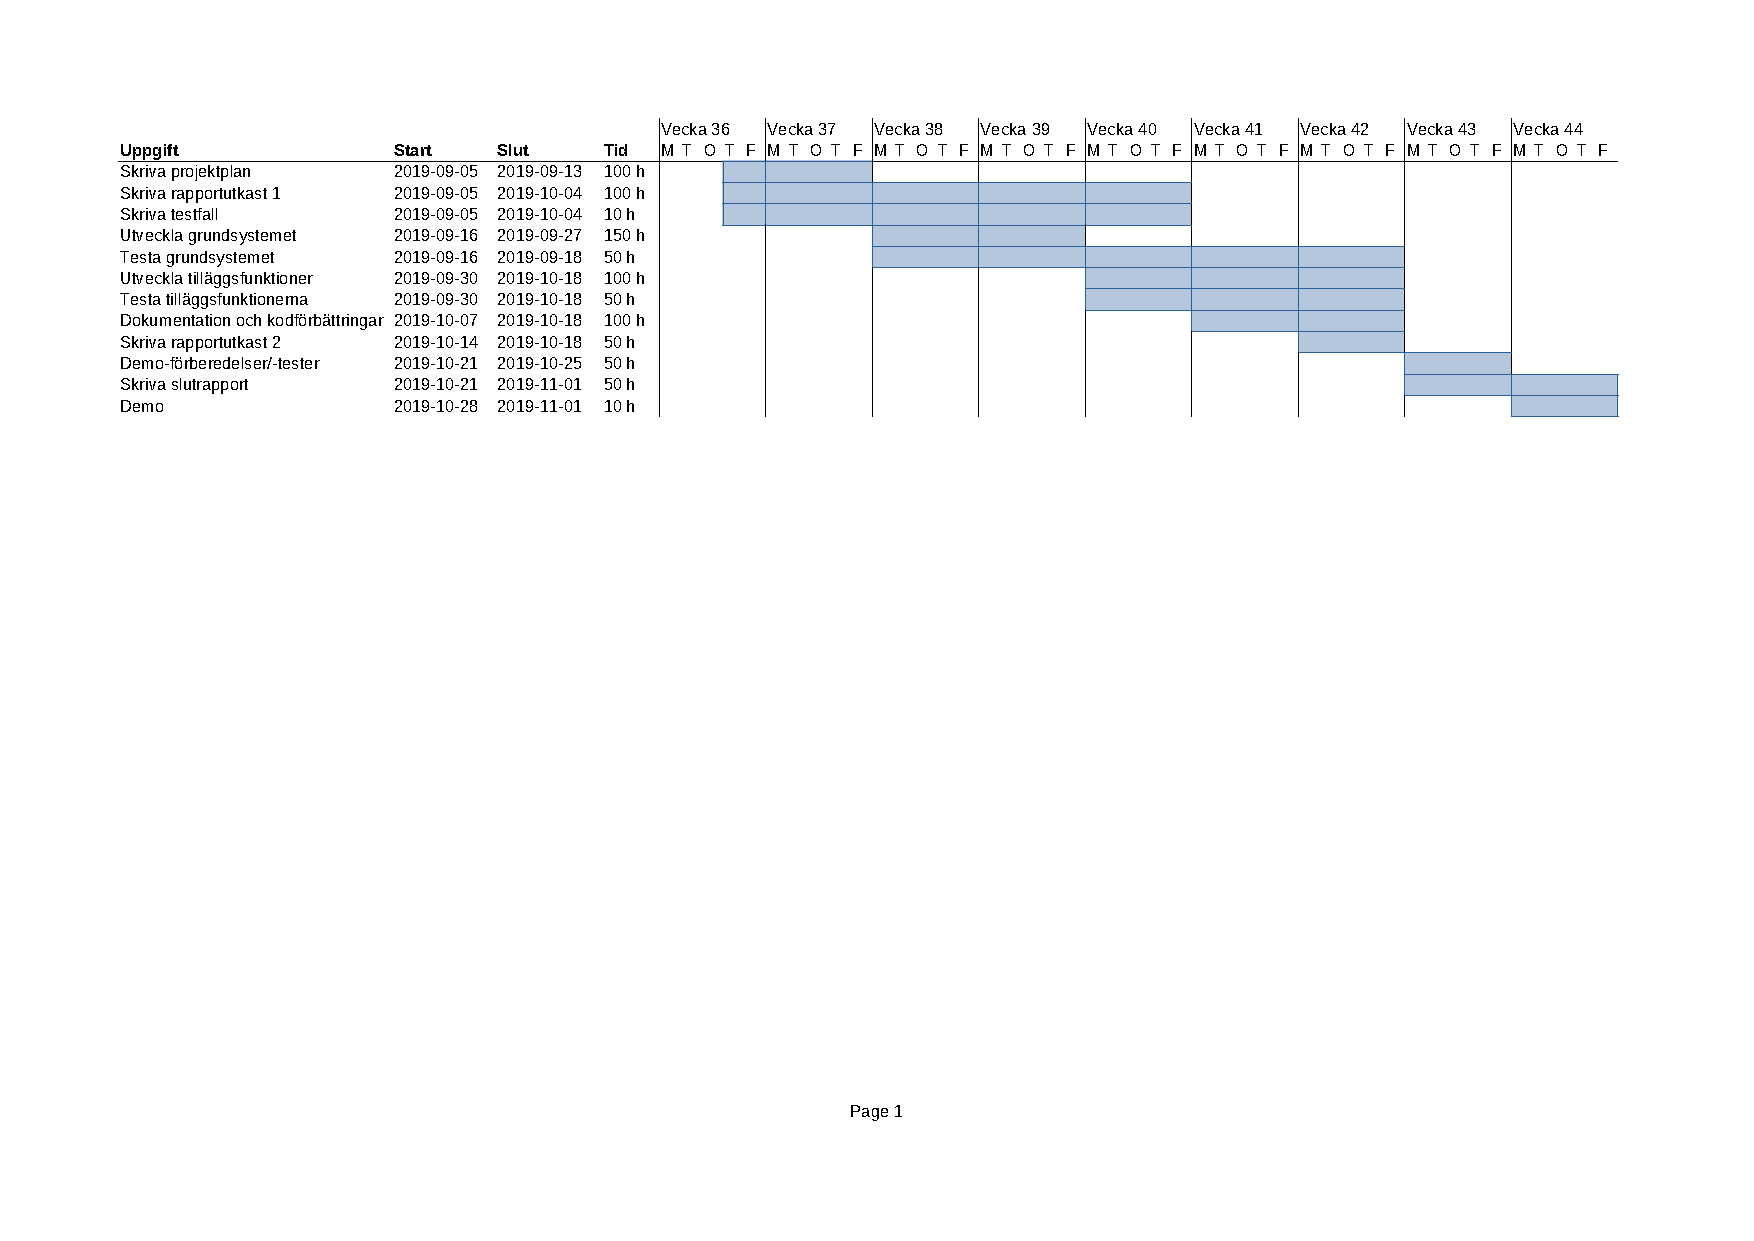
\includegraphics[trim={2cm 12cm 2cm 0}, clip, scale=0.525]{figurer/tidsplan.pdf}
\caption{En skiss på en Ganttbased tidsplan för projektet.}
\label{figur:tidsplan}
\end{figure}

\section{Mötesplan}
\label{sec:mötesplan}

Gruppen planerar att ha veckomöte varje torsdag kl. 10:00 - 11:00 i projektrum EG-4213. På dessa möten förväntas samtliga gruppmedlemmar deltaga.

Preliminär tid och plats för planerade veckomöten visas i tabell \ref{tabell:möten}. Utöver dessa möten ska gruppen, vid behov, tillkalla extramöten. Tid och plats för dessa möten bestäms gemensamt av gruppmedlemmarna.

\begin{table}
\centering
\begin{tabular}{| l | l | l | l |} 
\hline
\textbf{Vecka} & \textbf{Datum} & \textbf{Tid} & \textbf{Plats} \\ \hline
36 & 2019-09-05 & 10:00 - 11:00 & EG-4213 \\ \hline
37 & 2019-09-12 & 10:00 - 11:00 & EG-4213 \\ \hline
38 & 2019-09-19 & 10:00 - 11:00 & EG-4213 \\ \hline
39 & 2019-09-26 & 10:00 - 11:00 & EG-4213 \\ \hline
40 & 2019-10-03 & 10:00 - 11:00 & EG-4213 \\ \hline
41 & 2910-10-10 & 10:00 - 11:00 & EG-4213 \\ \hline
42 & 2019-10-17 & 10:00 - 11:00 & EG-4213 \\ \hline
43 & 2019-10-24 & 10:00 - 11:00 & EG-4213 \\ \hline
44 & 2019-10-31 & 10:00 - 11:00 & EG-4213 \\ \hline
\end{tabular}
\caption{Mötesplan för hela projektperioden. Utöver dessa möten kan gruppen besluta om extramöten.}
\label{tabell:möten}
\end{table}


\section{Kommunikationsplan}
\label{sec:kommunikationsplan}


\subsection*{Extern kommunikation}
% \label{sec:extern-kommunikation}

Den externa kommunikationen sker mestadels skriftligt genom möteskallelser, mötesprotokoll, projektplan och projektrapport riktade till kunden. Även munt-lig kommunikation till kunden kan komma att ske. Tabell \ref{tabell:kommunikationsplan} visar en sammanställ-ning av kommunikationsplanen för projektet.

\begin{table}[t]
\centering
\begin{tabular}{| l | l | l | l |}
\hline
\textbf{Vad}           & \textbf{Datum} & \textbf{Mottagare}    & \textbf{Hur}       \\ \hline
Mötesprotokoll (v. 36) & 2019-09-06   & Projektgrupp och kund & Lägg upp på Canvas \\ \hline
Kallelse möte  (v. 37) & 2019-09-11   & Projektgrupp och kund & Lägg upp på Canvas \\ \hline
Mötesprotokoll (v. 37) & 2019-09-13   & Kund                  & Lägg upp på Canvas \\ \hline
Projektplan            & 2019-09-13   & Projektgrupp och kund & Lägg upp på Canvas \\ \hline
Kallelse möte  (v. 38) & 2019-09-18   & Projektgrupp och kund & Lägg upp på Canvas \\ \hline
Mötesprotokoll (v. 38) & 2019-09-20   & Projektgrupp och kund & Lägg upp på Canvas \\ \hline
Kallelse möte  (v. 39) & 2019-09-25   & Projektgrupp och kund & Lägg upp på Canvas \\ \hline
Mötesprotokoll (v. 39) & 2019-09-27   & Projektgrupp och kund & Lägg upp på Canvas \\ \hline
Kallelse möte  (v. 40) & 2019-10-02   & Projektgrupp och kund & Lägg upp på Canvas \\ \hline
Mötesprotokoll (v. 40) & 2019-10-04   & Projektgrupp och kund & Lägg upp på Canvas \\ \hline
Kallelse möte  (v. 41) & 2019-10-09   & Projektgrupp och kund & Lägg upp på Canvas \\ \hline
Mötesprotokoll (v. 41) & 2019-10-11   & Projektgrupp och kund & Lägg upp på Canvas \\ \hline
Kallelse möte  (v. 42) & 2019-10-16   & Projektgrupp och kund & Lägg upp på Canvas \\ \hline
Mötesprotokoll (v. 42) & 2019-10-18   & Projektgrupp och kund & Lägg upp på Canvas \\ \hline
Kallelse möte  (v. 43) & 2019-10-23   & Projektgrupp och kund & Lägg upp på Canvas \\ \hline
Mötesprotokoll (v. 43) & 2019-10-25   & Projektgrupp och kund & Lägg upp på Canvas \\ \hline
Kallelse möte  (v. 44) & 2019-10-30   & Projektgrupp och kund & Lägg upp på Canvas \\ \hline
Mötesprotokoll (v. 44) & 2019-11-01   & Projektgrupp och kund & Lägg upp på Canvas \\ \hline
Projektrapport         & 2019-11-01   & Kund                  & Lägg upp på Canvas \\ \hline
\end{tabular}
\caption{Kommunikationsplan för projektet.}
\label{tabell:kommunikationsplan}
\end{table}

\subsection*{Intern kommunikation}
% \label{sec:intern-kommunikation}

För den interna kommunikationen används olika medium för olika typer av information.

\begin{description}
 \item [Canvas] Kallelser till veckomöten samt mötesprotokoll ska laddas upp på Can-vas.
 \item [Issue-funktionen på GitHub] För buggrapportering, frågor rörande doku-mentation och andra tekniska saker ska Issue-funktionen på GitHub använ-das.
 \item [Messenger-chat] Kort information, t.ex. ett planerat extramöte eller frågor till hela gruppen, ska kommuniceras via en Messenger-chat.
\end{description}

För övrig intern kommunikation ska e-post användas.

\section{Kvalitetsplan}
\label{sec:kvalitetsplan}

Kvalitén på produkten verifieras genom \textit{tester}.

Under projektets gång kommer det att utföras enhetstester för att testa de minsta delarna i systemet, funktionella tester på olika delar av systemet för att testa dess funktionalitet, prestandatester för att fastställa systemets prestanda och kapacitet, och slutligen användartester för att upptäcka förbättringar av systemet utifrån ett användarperspektiv.

Kvalitén på elektriska komponenter och övrig hårdvara kan verifieras genom tester med mätutrustning, medan en IDE (eng. \textit{Integrated Design Environment}) kan användas för att verifiera kvalitén på mjukvaran. Hur väl hård- och mjuk-varan fungerar ihop verifieras genom funktionstester och användartester.

Utifrån de krav som specificeras i systembeskrivningen (se avsnitt \ref{sec:systemöversikt}) skrivs ett \textit{testfall} som testar om kravet är uppfyllt. Varje testfall består av följande data:

\begin{description}
  \item [ID] Ett unikt ID på formen TXnnnvm, där X är E, F, P eller A för enhetstest, funktionellt test, prestandatest respektive användartest, nnn är ett num-mer mellan 0 och 999 tilldelat i den ordning testfallen skapats, och m är versionsnummret. Exempelvis är TF012v3 den tredje versionen av det tolfte funktionella testfallet.
  \item [Namn] Ett namn som tydligt beskriver vad testfallet ska testa.
  \item [Beskrivning] En beskrivning av testfallet. Beskrivningen ska beskriva syftet med testfallet, vilken komponent som testas, vilket eller vilka krav som testas samt eventuella tekniska förutsättningar för att genomföra testet.
  \item [Teststeg] De steg som måste utföras för att utföra testfallet.
  \item [Förväntat resultat] Beskrivning av det förväntade resultatet för testfallet.
\end{description}

Eftersom kvalitén på produkten verifieras genom tester är det viktigt att kvalitén på testfallen och utförandet av de är mycket hög. För att säkerställa detta ska alla testfall som skapas tilldelas status \textit{Utkast}. Testfallet kan sedan skickas vidare till \textit{granskning}. Granskningen ska ske av åtminstone en (1) person och personen får inte ha varit inblandad i skrivandet av testfallet. Testfallet kan antingen bli \textit{godkänt} eller \textit{avfärdat}. Om testfallet blir godkänt ändras dess status till \textit{Klar för test} och det får köras. Ett föråldrat eller inaktuellt testfall kan skickas tillbaka till granskning. Om testfallet däremot blir avfärdat måste det revideras och sedan åter skickas till granskning. De två reglerna för att skapa och köra testfall är följande: (1) endast testfall med status Utkast får redigeras och (2) endast testfall som har blivit granskade och godkända får köras.

\begin{figure}[h]
  \centering
  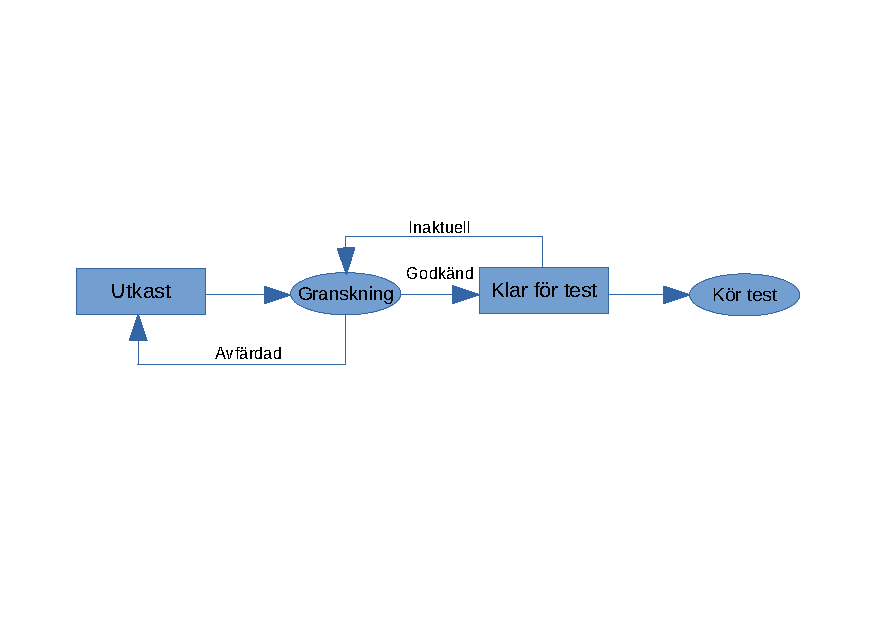
\includegraphics[trim={0 4cm 0 3cm}, clip, scale=0.8]{figurer/testrutin.pdf}
  \caption{Vår rutin kring att skriva och genomföra testfall.}
\end{figure}

Resultatet av samtliga körda tester ska sammanställas i en testresultat-fil på fjärrarkivet. I testresultatfilen ska följande fält, varav det sista är frivilligt, fyllas i:

\begin{description}
  \item [Datum] Datum för utförandet av testet.
  \item [ID] Testfallets unika ID.
  \item [Namn] Testfallets namn.
  \item [Hårdvara] Hårdvara som använts vid utförandet av testet.
  \item [Mjukvara] Version på mjukvaran som använts vid utförandet av testet.
  \item [Faktiskt resultat] Beskrivning av det faktiska resultatet. Om det faktiska resul-tatet är detsamma som det förväntade resultatet ska \textit{Som förväntat} anges.
  \item [Status] Status på testet. \textit{G} ska anges om testet blev godkänt, det vill säga om det faktiska resultatet blev det samma som det förväntade resultatet, och \textit{M} om testet misslyckades.
  \item [Kommentar] Eventuella kommentarer, till exempel analys av testfallet. Detta fält är frivilligt.
\end{description}

Resultatet av samtliga körda tester ska analyseras och diskuteras åtminstone på det veckovisa gruppmötet. Då ska även bestämmas vilka tester som i första hand ska köras innan nästa möte.

\subsection*{Integrering av utveckling och testning}

Eftersom vår projektgrupp består av endast fem personer kan vi, på ett effektivt sätt, integrera testning med utveckling. Vi väljer att jobba efter en cirkulär modell där testningen blir en naturlig del av utvecklingsfasen, ty så snart en funktion utvecklats, testas den. På så sätt kan buggar hittas och lösas tidigt i utvecklingsfasen.

\begin{figure}[h]
  \centering
  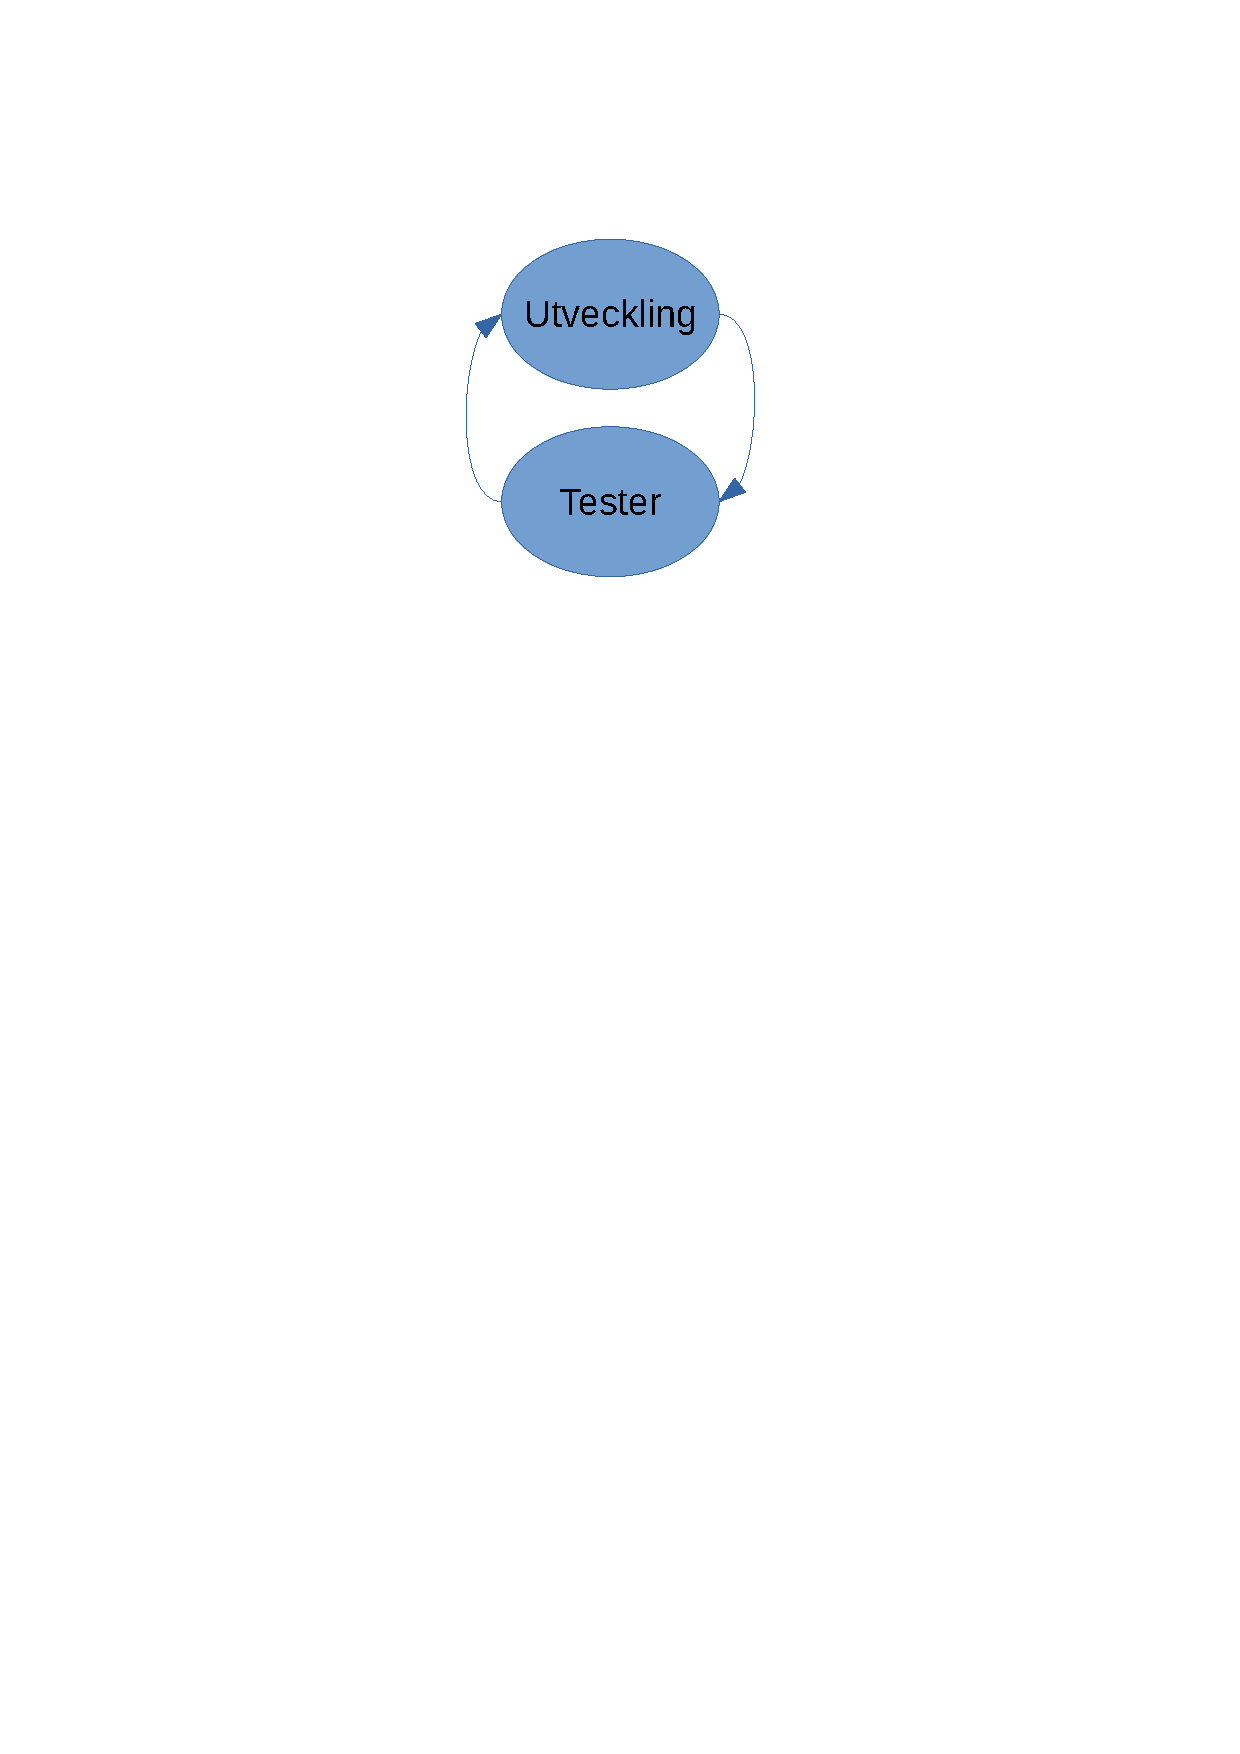
\includegraphics[trim={0 19cm 1cm 3cm}, clip, scale=0.5]{figurer/arbetsrutin.pdf}
  \caption{Vår arbetsrutin. Utvecklarna får direkt återkoppling från testresultaten och kan lösa buggar tidigt i utvecklingsfasen.}
\end{figure}

\newpage

\begin{thebibliography}{999}
\label{sec:referenser}
\bibitem{sverigesRadio}
L. Jungefeldt. ``Säkerhetsbranschen växer i Sverige.`` sverigesradio.se.
https://sverigesradio.se/sida/artikel.aspx?programid=83\&artikel=7284631 (hämtad 2019-09-07)
\bibitem{vibrationsSensor}
``Vibration Sensor`` espruino.com.
https://www.espruino.com/Vibration (hämtad 2019-09-12)
\end{thebibliography}

\end{document}
